\section{Analysis of SD Under Cached Offloading}
\label{sec:model}

This section analyzes when and why speculative decoding underperforms under cached offloading, and under what conditions it can succeed. We first derive a memory threshold $M^*$ that marks a phase transition in SD effectiveness (\S\ref{subsec:threshold}). We then identify two practical barriers that prevent SD from reaching its potential even above $M^*$: Observation~1 reveals that cache hits do not deliver HBM-speed execution due to path overhead (\S\ref{subsec:obs1}), and Observation~2 shows that transient working-set overflow triggers cascading evictions that amplify expert-transfer cost (\S\ref{subsec:obs2}). Section~\ref{subsec:implications} maps these findings to the design requirements addressed in Section~\ref{sec:design}.

\subsection{Memory Threshold $M^*$}
\label{subsec:threshold}

The GPU memory budget $M_{\mathrm{GPU}}$ must accommodate non-expert components (non-MoE model weights, KV cache, the draft model, and activations), which together occupy $M_{\mathrm{base}}$ bytes. The remaining memory $C = M_{\mathrm{GPU}} - M_{\mathrm{base}}$ is available for expert caching. Distributing this budget uniformly across the $L_{\mathrm{off}}$ offloaded MoE layers yields
\begin{equation}
\label{eq:slots}
S = \left\lfloor \frac{M_{\mathrm{GPU}} - M_{\mathrm{base}}}{L_{\mathrm{off}} \cdot m_e} \right\rfloor
\end{equation}
cache slots per layer, where $m_e$ is the per-expert memory footprint.

For SD to benefit from caching, the cache must be large enough to hold SD's steady-state working set: $S \ge \bar{\wsd}$. Rearranging Equation~\ref{eq:slots} yields the minimum GPU memory required:
\begin{equation}
\label{eq:mstar}
M^* = M_{\mathrm{base}} + L_{\mathrm{off}} \cdot \bar{\wsd} \cdot m_e.
\end{equation}
Below $M^*$, the cache cannot accommodate $\bar{\wsd}$ experts per layer; a significant fraction of SD's expert accesses miss the cache and fall back to PCIe. Because a single cache miss costs $t_{\mathrm{miss}} \approx 0.378$~ms (Section~\ref{sec:background}), these misses accumulate across $L_{\mathrm{off}}$ layers each step, and the resulting transfer cost offsets SD's multi-token verification benefit. Above $M^*$, most expert accesses are served from HBM, and the PCIe transfer cost is mitigated, though not eliminated, as we show in Observation~2.

In our configuration, $L_{\mathrm{off}}=26$ layers are offloaded, $\bar{\wsd}\approx 17$ in steady state, and $m_e=9.44$~MB, giving $M^*\approx 40$~GiB. Figure~\ref{fig:phase} validates this prediction experimentally. Below $M^*$, all four configurations (AR, SD, AR with \sysname, and SD with \sysname) remain flat at 1--5~tok/s; SD provides no benefit over AR regardless of system-level optimizations. Above $M^*$, SD with \sysname rises sharply to 19~tok/s while AR with \sysname reaches only 6.5~tok/s. The phase transition occurs precisely at the predicted $M^*\approx 40$~GiB, confirming that cache capacity is the gating factor for SD effectiveness.

\begin{figure}[t]
\centering
% TODO: generate fig_phase_transition.pdf from phase transition data
\includegraphics[width=\columnwidth]{figures/BriskMoE}
\caption{Memory-dependent phase transition in SD effectiveness. Below the derived threshold $M^*\approx 40$~GiB, SD provides no benefit (SD+\sysname $\approx$ AR+\sysname). Above $M^*$, SD with \sysname rises sharply to 19~tok/s while AR with \sysname plateaus at ${\sim}6.5$~tok/s.}
\Description{Line chart with four curves (AR, SD, AR+BriskMoE, SD+BriskMoE) across GPU memory budgets from 24 to 44 GiB. All curves are flat below 40 GiB; SD+BriskMoE rises sharply above 40 GiB.}
\label{fig:phase}
\end{figure}

$M^*$ delineates the applicability boundary of \sysname: the remainder of this section, and the design in Section~\ref{sec:design}, assumes $M_{\mathrm{GPU}} \ge M^*$. Even at 44~GiB, the setting of our motivating example (Figure~\ref{fig:motivation}), cached SD throughput reaches only 5.81~tok/s, far below the potential suggested by SD's ${\sim}2.5$~tok/step acceptance rate. Since $S \ge \bar{\wsd}$ at this budget, the bottleneck is not insufficient cache capacity. The following two observations reveal that the problem lies in the cache access path itself.

\subsection{Observation 1: Cache-Hit Path Overhead}
\label{subsec:obs1}

When $M_{\mathrm{GPU}} \ge M^*$, most expert accesses hit the cache and $T_{\mathrm{load}}$ is mitigated. One might expect cache hits to be served at HBM speed, making the MoE kernel the sole bottleneck. Profiling reveals otherwise. Recall from \S\ref{subsec:cached} that the scratchpad baseline decomposes per-layer latency into
\begin{equation}
\label{eq:decomp}
T_{\mathrm{layer}} = \underbrace{T_{\mathrm{sync}} + T_{\mathrm{copy}} + T_{\mathrm{kernel}}}_{\text{$\eta$-independent floor}} + \underbrace{N_{\mathrm{miss}} \cdot t_{\mathrm{miss}}}_{\text{$\eta$-dependent}},
\end{equation}
where $T_{\mathrm{sync}}$ is the cost of GPU--CPU synchronization for cache lookup (\texttt{unique}$\to$\texttt{tolist} and dictionary operations), $T_{\mathrm{copy}}$ is the HBM-to-HBM scratchpad copy that assembles all $W$ accessed experts into a contiguous buffer (required for both hits and misses), and $T_{\mathrm{kernel}}$ is the fused MoE kernel time. Crucially, $T_{\mathrm{sync}}$ and $T_{\mathrm{copy}}$ are incurred for every accessed expert regardless of whether it hits the cache, so increasing $\eta$ reduces only the last term.

\begin{figure}[t]
\centering
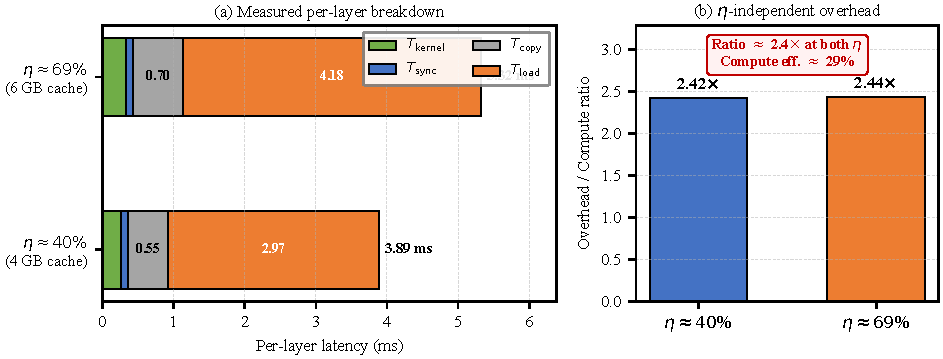
\includegraphics[width=\columnwidth]{figures/fig_latency_breakdown.pdf}
\caption{Per-layer latency decomposition under scratchpad-mode caching at two hit rates ($\eta\approx 40\%$ with 4~GB cache and $\eta\approx 69\%$ with 6~GB cache). (a)~Stacked breakdown: although absolute component values differ, the non-load overhead scales proportionally with the kernel. (b)~The overhead-to-compute ratio $(T_{\mathrm{copy}}+T_{\mathrm{sync}})/T_{\mathrm{kernel}} \approx 2.4\times$ is constant across $\eta$, confirming the $\eta$-independent performance floor at 29\% compute efficiency.}
\Description{Two panels: (a) stacked horizontal bars comparing per-layer breakdown at two hit rates; (b) two vertical bars showing overhead-to-compute ratio of 2.42x and 2.44x at the two hit rates.}
\label{fig:breakdown}
\end{figure}

Figure~\ref{fig:breakdown} profiles the scratchpad-mode baseline running SD at two cache sizes (4~GB and 6~GB within a 44~GiB budget). Panel~(b) shows the key finding: the overhead-to-compute ratio $(T_{\mathrm{copy}} + T_{\mathrm{sync}}) / T_{\mathrm{kernel}} \approx 2.4\times$ is constant across $\eta$. This $\eta$-independent ratio means that even at $\eta \to 1$ (all hits, $N_{\mathrm{miss}} = 0$), the cache-hit path overhead would still consume ${\sim}71\%$ of the residual per-layer time, yielding only 29\% compute efficiency. The design implication is that the system must \emph{unblock} the cache-hit path by eliminating $T_{\mathrm{copy}}$ and reducing $T_{\mathrm{sync}}$.

\subsection{Observation 2: Transient Working-Set Overflow}
\label{subsec:obs2}

The threshold $M^*$ is derived from the steady-state working set $\bar{\wsd}\approx 17$, ensuring $S \ge \bar{\wsd}$. However, SD's per-step working set fluctuates: the per-step union averages ${\sim}19.3$ experts and peaks at ${\sim}26.9$ (Figure~\ref{fig:motivation}a). When $W_{\mathrm{step}} > S$ in a given step, the overflow experts must be fetched from host memory, incurring a direct per-step penalty of
\begin{equation}
\label{eq:overflow}
\Delta T_{\mathrm{step}} = L_{\mathrm{off}} \cdot \max(0,\; W_{\mathrm{step}} - S) \cdot t_{\mathrm{miss}}.
\end{equation}
Table~\ref{tab:overflow} quantifies this cost. At $S=17$, a mean-case step ($W_{\mathrm{step}}=19$) incurs 19.6~ms of additional transfer, roughly 20\% of a decode step at 10~tok/s, while a peak step ($W_{\mathrm{step}}=27$) incurs 98.3~ms, nearly doubling the step time.

\begin{table}[t]
\caption{Per-step overflow cost at $S=17$ cache slots, $L_{\mathrm{off}}=26$ layers, $t_{\mathrm{miss}}=0.378$~ms.}
\label{tab:overflow}
\centering
\small
\begin{tabular}{cccc}
\toprule
$W_{\mathrm{step}}$ & $N_{\mathrm{overflow}}$ & Per-layer $\Delta T$ & Total $\Delta T_{\mathrm{step}}$ \\
\midrule
17 (steady state) & 0 & 0~ms & 0~ms \\
19 (mean) & 2 & 0.76~ms & 19.6~ms \\
27 (peak) & 10 & 3.78~ms & 98.3~ms \\
\bottomrule
\end{tabular}
\end{table}

The damage extends beyond a single step. Overflow forces eviction of cached experts to make room for the new arrivals. Because expert routing exhibits high temporal locality (approximately $\alpha \approx 15/17 \approx 0.88$ of a step's experts are reused in the next step), evicted experts are likely to be needed again shortly. When they are, the system suffers another miss, evicts yet another expert, and the cycle repeats. A single overflow event thus propagates across $O(1/(1-\alpha)) \approx 8$ subsequent steps, amplifying the initial transfer penalty into a sustained throughput degradation.

\begin{figure}[t]
\centering
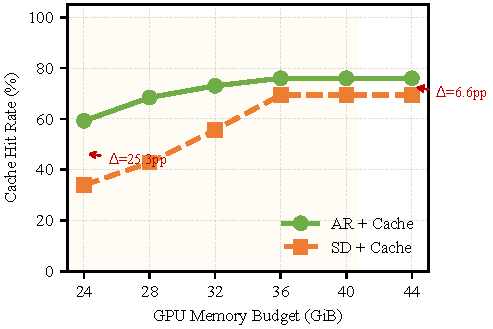
\includegraphics[width=\columnwidth]{figures/fig_hitrate_sweep.pdf}
\caption{Expert-cache hit rate under AR and SD across six GPU memory budgets. SD consistently achieves a lower $\eta$ than AR due to its larger per-step working set. The gap persists even at 44~GiB, confirming that transient overflow continuously degrades cache coverage.}
\Description{Dual-line chart showing cache hit rate versus GPU memory budget. The AR line is consistently above the SD line across all budgets.}
\label{fig:hitrate}
\end{figure}

Figure~\ref{fig:hitrate} confirms this effect: at every memory budget, $\eta_{\mathrm{SD}} < \eta_{\mathrm{AR}}$. Even at 44~GiB where $S \ge \bar{\wsd}$, the gap remains 6.6 percentage points (76.0\% vs.\ 69.4\%), because per-step fluctuations continuously trigger evictions. The design implication is that the system must \emph{protect} the cache from transient overflow by pre-staging experts before verification begins.

\subsection{Design Implications}
\label{subsec:implications}

The analysis yields one applicability condition and two design requirements for \sysname, as summarized in Table~\ref{tab:obs_design}.

\begin{table}[t]
\caption{Mapping from analysis findings to \sysname design.}
\label{tab:obs_design}
\centering
\small
\begin{tabular}{lll}
\toprule
Finding & Bottleneck & Design Response \\
\midrule
$M^*$ threshold & $S < \bar{\wsd}$ $\Rightarrow$ PCIe-bound & Applicability condition \\
Obs.~1: Hit-path overhead & $T_{\mathrm{copy}},\;T_{\mathrm{sync}}$ & \emph{Unblock} (\S\ref{sec:design}) \\
Obs.~2: Transient overflow & cascade miss $\Rightarrow$ $T_{\mathrm{load}}\!\uparrow$ & \emph{Protect} (\S\ref{sec:design}) \\
\bottomrule
\end{tabular}
\end{table}

$M^*$ is the necessary condition for SD to benefit from expert caching. Above $M^*$, Observation~1 requires removing the cache-path bottlenecks that prevent cache hits from achieving HBM-speed execution (\emph{Unblock}), and Observation~2 requires maintaining cache coverage under SD's fluctuating working set (\emph{Protect}). Section~\ref{sec:design} addresses both.
